\chapter{Project Description}
\label{project_description}

\section{Requirements}
\noindent Our proposed solution will feature the following: 
\begin{itemize}[noitemsep]
	\item Low power consumption – The system will focus on event-driven updates in order to conserve as much energy as possible and prolong time between sensor battery replacements.
	\item Ease of installation – With a wireless sensor network approach, this system will avoid cabling installation. Also, dynamic routing makes it possible to install sensors in a plug-and-play fashion.
	\item Reliability – The routing protocol focuses on reaching the control center keeping several alternate paths ready in case of connectivity loss.
	\item Error detection – By keeping track of each device's power level on every message, sensors running low on battery can be quickly identified and get a replacement before losing connectivity.
	\item Fast reaction times – The system is designed to notify of parking status changes within 5 to 10 seconds.
\end{itemize}

\section{Topology}
The two scenarios where this solution could be applied would be mainly in parking lots, and multi-story car parks, but also curb parking spaces.
In order to communicate the status of the parking spaces, Crossbow MicaZ motes are programmed with one of three roles (see figure \ref{fig:topology}):
\begin{enumerate}
	\item Sensor - Mote running on two AA batteries equipped with a light sensor and encased in a protective shell that is fixed to the floor or pavement.
	It is responsible for monitoring parking space occupancy and inform its immediate gateway of a status change.
	\item Gateway - Mote connected to a power source in an elevated position (e.g. a street lamp). 
	It provides network access to the sensors by forwarding their status messages towards the control center. 
	It also builds a distance-based routing table that consists of neighbor gateway addresses and their distance to the control center.
	\item Control Center (CC) - Mote connected to a computer or web server. This device will receive and process all status messages from every gateway. 
	It also provides statistical information and GUI for the parking lot operator and information to be printed in an outdoor display for the drivers.
\end{enumerate}

\begin{figure}
    \centering
    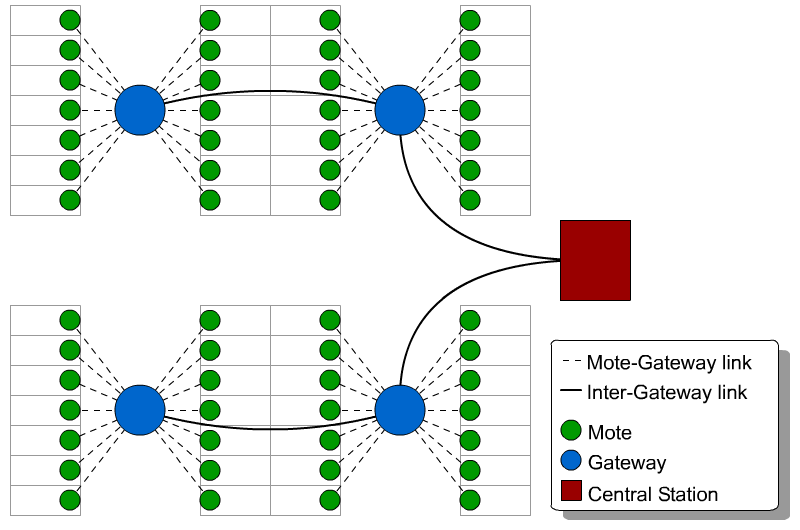
\includegraphics[width=15cm]{images/Topology_General.png}
	\vspace{-1.5em}
    \caption{Example topology of a small parking lot}
    \vspace{-1.5em}
    \label{fig:topology}
\end{figure}

\section{Routing}
The routing protocol proposed is dynamic and meant to ease installation in a plug-and-play fashion. 
The objectives of our implementation is to develop a simple, yet effective and fast route selection. 
It should provide quick reaction times and backup path switch-over in case of gateway saturation or connectivity loss.
Lastly, it should allow new sensors or gateways to be added to the network with as little configuration effort as possible, if any.
We decided a protocol mix of Dijkstra and rumor routing could meet all these requirements.

\bigskip
\subsection{Rumor Routing}
Each node has its neighbor list, and an events table, with forwarding information to all the events it knows. 
After a node witnesses an event, it sends a special long-lived packet to the network known as an agent.
The agent travels around the network hopping from node to node creating a path towards the event.
Each agent contains an events table, including the routing information for all events it knows.
Since an event happens in a zone, composed of several or many nodes, it’s possible more than one agents are created from the zone and moving in the network.
 An agent's routing table will be updated if there’s a shorter path to an event within the routing table of the node it is visiting. 
Also, the routing table of the currently visited node will be updated if its route to an event is more costly than the agent’s. 

Once there are events, agents and paths on the network, any node may query for a particular event. 
If it knows the route to the event, it will transmit the query. 
Otherwise, the query will be sent and propagated in a random direction until the query reaches a node with a route to the event. 

Properties
\begin{itemize}
	\item Power saving, improves network longevity.
	\item Robust in dealing node failure.
	\item Tunable, allow tradeoff between setup overhead and delivery reliability.
\end{itemize}
 Assumptions
\begin{itemize}
	\item No coordinate system is available so location information is not known by nodes.
	\item Static topology.
\end{itemize}

\subsection{Dijkstra's algorithm for best path selection}

Disadvantages
\begin{itemize}
	\item Looking for the shortest path by flooding consumes a lot of energy.
	\item Flooding increases the chance of collision.
	\item This application only requests a small amount of data back (ACK).
\end{itemize}

How have we combined them.
\bigskip

The first device in the network should be the control center. 
Afterwards, the gateways can be installed and turned on.
Upon booting, the gateways will start exchanging routing information and converge once a wireless path towards the CC is found.
If at least one gateway is online, sensors can be installed. 
These will attempt to discover any gateway within range and create an ordered list of gateways based signal strength.
When a parking status event triggers a message, the sensor will attempt to send it to the nearest gateway for forwarding. 
If this gateway fails to process the packet, the sensor is notified and will then repeat the process with the next gateway on its list.


%\bigskip
%\noindent \textsl{[...]"Some text in italics"}

